\chapter{Recursos Energéticos y la Producción de Electricidad.}

\section{Introducción.}
	\begin{itemize}
		\item[-] \textit{\textbf{Recursos energéticos:}}
			principalmente son combustibles fósiles y nuestra sociedad se ha
			hecho extraordinariamente dependiente de ellos para su desarrollo.
		
		\item[-] \textit{\textbf{Combustibles fósiles:}}
			comprenden principalmente el petróleo y sus derivados (gasolinas,
			gasóleos, gases licuados del petróleo, etc.), el gas natural, el carbón mineral y el uranio.\linebreak
			Al principio de la explotación de estos recursos, se consideraban ilimitados y su impacto
			ambiental era despreciable.
			
		\item[-] \textit{\textbf{Consumo masivo de hidrocarburos:}} está produciendo alteraciones en la atmósfera a nivel mundial
		por la emisión de gases de efecto invernadero, originando un calentamiento global y un cambio
		climático.
		
		\item[-] \textit{\textbf{Esquema de consumo energético actual:}} no es sustentable por:
		\begin{itemize}
			\item[-] \textit{Razones económicas:} próxima escasez de hidrocarburos.
			\item[-] \textit{Razones ecológicas:} alteración de la atmósfera y el suelo.
		\end{itemize}
		Es imperativo el \textbf{desarrollo de nuevas alternativas energéticas} más eficientes y menos agresivas contra el medio ambiente:
		\begin{itemize}
			\item[-] Incremento de las fuentes de energía renovable, consideradas como inagotables.
			\item[-] Resurgimiento de la energía nuclear.
		\end{itemize}
	\end{itemize}
	
		
\section{Fuentes de energía no renovable.}
	\begin{itemize}
		\item[-] \textbf{\textit{Definición:}} 
			energía que está almacenada en cantidades fijas, comúnmente en
			el subsuelo. A medida que se consume un recurso no renovable, se va agotando.
		\item[-] \textbf{\textit{Reservas:}}
			sujetas a la factibilidad técnica y económica de su explotación, al
			descubrimiento de nuevos yacimientos y al ritmo de extracción y consumo.
	\end{itemize}
	
		\subsection{Fuentes de energía fósil.}
			Se llama energía fósil la que se obtiene de la combustión (oxidación) de ciertas substancias que,
			según la geología, se produjeron en el subsuelo a partir de la acumulación de grandes cantidades de
			residuos de seres vivos, hace millones de años. Son los siguientes recursos:
			\begin{itemize}
				\item[-] \textit{Petróleo y derivados:}
					el petróleo es una mezcla de una gran variedad de hidrocarburos
					(compuestos de carbono e hidrógeno) en fase líquida, mezclados con una gran variedad de
					impurezas. Por destilación y otros procesos, se obtienen las diversas gasolinas, el diésel, etc.
				\item[-] \textit{Gas natural:} 
					está compuesto principalmente por metano y corresponde a la
					fracción más ligera de los hidrocarburos, por lo que se encuentra en los yacimientos en forma
					gaseosa.
				\item[-] \textit{Carbón mineral:}
					es principalmente carbono, también de origen fósil, que
					se encuentra en grandes yacimientos en el subsuelo.
			\end{itemize}
			
		\subsection{Fuentes de energía nuclear.}
			Son aquellas que provienen de la desintegración de átomos mediante fisión o la fusión de isótopos para producir energía.
			\begin{itemize}
				\item[-] \textit{Uranio:}
					elemento radiactivo natural. Se encuentra en la naturaleza en casi
					todas las rocas y suelos.
				\item[-] \textit{Torio:}
					tiene usos muy similares al Uranio.
				\item[-] \textit{Energía de fusión nuclear:} 
					pretende imitar el comportamiento de las reacciones que se producen en el Sol. Fusionando un isótopo de Deuterio con otro de Tritio se obtiene un átomo de Helio, un neutrón y energía.
			\end{itemize}
		
\section{Fuentes de energía renovable.}
		Se llama energía renovable la que puede explotarse ilimitadamente, es decir, su cantidad disponible (en
		la Tierra) no disminuye a medida que se aprovecha. La principal fuente de energía renovable es el Sol:
		\begin{itemize}
			\item[-]
				Es una esfera gaseosa, cuyos componentes principales son el hidrógeno, el helio y el carbono.
				Su masa es 330.000 veces la de la Tierra.
			\item[-]
				Se comporta como una perfecta central nuclear y en su seno se desarrollan reacciones termonucleares
				de fusión de núcleos de hidrógeno en helio.
			\item[-]
				En su núcleo, fusiona 620 millones de toneladas métricas ($620\cdot10^9$ kg) de hidrógeno por segundo: $4 H\longrightarrow1 He$ + \textit{Energía.}
		\end{itemize}
		
		\indent Algunos datos sobre el efecto del Sol sobre la Tierra:
		\begin{itemize}
			\item[-]
				Como la masa del Sol es del orden de $2\cdot10^{30}$ kg y contiene el 30$\%$ de hidrógeno, si todo el hidrógeno solar se convirtiera en helio se obtendría una energía de $3.75\cdot10^{44}$ J.
			\item[-] 
				La Tierra recibe una irradiancia de $1370 \dfrac{\textit{W}}{\textit{m}^2}$ (constante solar) en la parte exxterna de la atmósfera, y como la distancia media del Sol a la Tierra es de $1.5\cdot10^{11}$ m, el Sol emita una radiación igual a:
				\[4\pi(1.5\cdot10^{11})^{2}\cdot1370 = 3.8\cdot10^{26}\dfrac{\textit{J}}{\textit{s}}\]
				La Tierra podrá alimentarse de radiaciones durante $3.13\cdot10^{10}$ años.
			\item[-] 
				No toda la radiación interceptada por la Tierra es absorbida; una fracción de la energía incidente es reflejada
				de regreso al espacio, principalmente por las nubes ($\simeq20\%$), por los constituyentes atmosféricos ($\simeq6\%$) y por la superficie terrestre ($\simeq4\%$).
			\item[-] 
				En la superficie terrestre llega una irradiancia alrededor de los $1.000 \dfrac{\textit{W}}{\textit{m}^2}$
		\end{itemize}
			
			\subsection{Energía solar.}
				Está constituida simplemente por la porción de la luz que emite el Sol y que es	interceptada por la Tierra. Puede ser:
				\begin{itemize}
					\item[-] \underline{Directa:}
						una de las aplicaciones de la energía solar es directamente como luz solar, por ejemplo, para la iluminación de recintos. En este sentido, cualquier ventana es un colector solar.
					\item[-] \underline{Térmica:}
						se denomina térmica la energía solar cuyo aprovechamiento se logra por medio del
						calentamiento de algún medio: agua o aceite. Pueden ser:
						\begin{itemize}
							\item[-] \textit{De baja temperatura:} 
								con colectores para producción de ACS (Agua Caliente Sanitaria).
							\item[-] \textit{De alta temperatura:} 
								centrales termosolares para producción de energía eléctrica mediante espejos parabólicos o con heliostatos con receptor central en torre.
						\end{itemize}
					\item[-] \underline{Fotovoltaica:}
						es el aprovechamiento de la energía solar por medio de células fotoeléctricas,
						capaces de convertir la luz en potencial eléctrico, sin pasar por un efecto térmico. El conjunto de
						células fotoeléctricas se denomina panel fotovoltaico. Se encuentra en las centrales fotovoltaicas.
				\end{itemize}
				
			\subsection{Energía eólica.}
				Es la energía que se extrae del viento que procede de la energía solar y del movimiento de rotación
				de la Tierra. La aplicación más importante es con la utilización de aerogeneradores en parque eólicos (\textit{onshore} y \textit{offshore}).
			\subsection{Energía de la biomasa.}
				\textit{Definición de biomasa:} conjunto de materiales de origen biológico, vegetal, animal o procedente de
				la transformación natural o artificial de estos materiales, utilizados para la producción de energía
				eléctrica o térmica.\\
				\indent Es un tipo de producción de energía gestionable. Depende de la disponibilidad de biomasa. Se utiliza en:	
				\begin{itemize}
					\item[-] Centrales térmicas de combustión de biomasa con turbinas de vapor.
					\item[-] Centrales térmicas de gasificación de biomasa con cogeneración:
					\begin{itemize}
						\item MACI (Motores Alternativos de Combustión Interna).
						\item Turbina de gas.
					\end{itemize}
				\end{itemize}
				
			\subsection{Energías marinas.}
				\begin{itemize}
					\item[-] \textit{Diferencia de temperatura oceánica (OTEC):} 
						Consiste en aprovechar la diferencia de temperatura que existe entre la superficie del océano (unos 20 \textdegree C o más en las zonas tropicales) y la correspondiente a unas decenas de metros debajo de la superficie (cercana a 4 \textdegree C).
					\item[-] \textit{Energía de las olas: central undimotriz:}
						También se puede aprovechar el vaivén de las olas del mar para generar energía eléctrica. Las olas son, a
						su vez, producidas en parte ,por el efecto del viento sobre el agua y por el movimiento rotacional de la Tierra.
					\item[-] \textit{Energía de las mareas: central mareomotriz:}
						Depende de la atracción gravitatoria del Sol y la Luna En algunas regiones costeras se dan unas mareas
						especialmente altas y bajas. La amplitud de la marea en algunos puntos de la Tierra puede alcanzar los 10 m.
					\item[-] \textit{Energía de las corrientes marinas:}
						A profundidades de 20 a 30 m existen unas corrientes marinas de baja velocidad (2 a 3 m/s) que dependen de
						los ciclos de las mareas.
					\item[-] \textit{Gradiente salino o Potencia osmótica:}
						Aprovechar la diferencia de salinidad entre el agua de los océanos y el agua de los ríos.
				\end{itemize}
				
			\subsection{Energía hidráulica.}
				Se obtiene a partir de caídas de agua, artificiales o naturales. Estrictamente, también esta es una forma derivada de la energía solar, porque el Sol provee la fuerza impulsora del ciclo hidrológico.\\
				\indent Se dividen en grandes y pequeñas centrales hidroeléctricas.
		
			\subsection{Hidrógeno. Pila de combustible.}
				El uso del hidrógeno como portador energético para complementar los mercados de la electricidad y
				combustibles líquidos presenta ventajas de versatilidad de fuentes de suministro, almacenamiento eficaz y
				bajas emisiones en los puntos de consumo.\\
				\indent La pila de combustible combina hidrógeno y oxígeno a través de una membrana de intercambio protónico,
				puede generar energía eléctrica obteniéndose como único residuo agua.\\
				\indent Para conseguir hidrógeno hay que consumir energía eléctrica. El hidrógeno se puede obtener:
				\begin{itemize}
					\item[-] \textit{Blanco:} en estado bruto en el subsuelo.
					\item[-] \textit{Verde:} del agua mediante electrolisis con energías renovables y biometano.
					\item[-] \textit{Rosa:} del agua mediante electrolisis con energía nuclear.
					\item[-] \textit{Gris:} del gas natural.
					\item[-] \textit{Azul:} del gas natural, pero se captura el $\textit{CO}_2$ residual.
					\item[-] \textit{Marrón:} del carbón.
				\end{itemize}
				Para transformar de vuelta el hidrógeno en electricidad hay dos métodos:
				\begin{itemize}
					\item[-] \textit{Grupo electrógeno:} utilizando un motor de combustión interna.
					\item[-] \textit{Pila de combustible:} $H_2 + \dfrac{1}{2}O_2 \longrightarrow H_2O$ + Calor + Energía Eléctrica.
				\end{itemize}
		
			\subsection{Energía geotérmica.}
				La energía geotérmica es un tipo de energía renovable que se basa en el aprovechamiento del calor
				que existe en el subsuelo de nuestro planeta. Es decir, utilizar el calor de las capas internas de la
				Tierra y con él genera energía.\\
				\indent La temperatura de la Tierra va a aumentando conforme descendemos y nos acercamos al núcleo
				terrestre. El gradiente térmico hace aumentar la temperatura del suelo entre 2 \textdegree C y 4 \textdegree C por cada 100 metros que descendemos. Hay diversas zonas del planeta donde este gradiente es mucho mayor y se debe
				a que la corteza terrestre es más delgada en ese punto.
		
\section{Combustibles fósiles.}
	\subsection{Reservas y recursos mundiales.}
		Las cantidades de materia prima energética que pueden aprovecharse para su transformación en energía útil en condiciones económicas rentables se denominan reservas (explotables). Cuando hay razones suficientes para la
		existencia de cantidades mayores, a estas se les denomina recursos (previsibles).\\
		\indent La evaluación de las reservas energéticas existentes en nuestro planeta se estimaban en\linebreak
 $33000\cdot10^{18}$ J, a los cuales habría que añadir $349395\cdot10^{18}$ J correspondientes a recursos de difícil explotación.

	\subsection{Evolución de las reservas de petróleo y gas.}
		\begin{center}
			\renewcommand{\arraystretch}{1.4}
			\begin{tabular}{ccccccc}
					\hline
						& \textbf{1984} & \textbf{1994} & \textbf{2004} & \textbf{2020} & \textbf{Duración Reservas} & \textbf{Evolución R/P}\\
					\hline
					Petróleo - $10^9$ barriles & 761 & 1017 & 1185 & 1732 & \multirow{2}{*}{42 años} & \multirow{2}{*}{31 a 42 años}\\
					Petróleo - $\%$ & 100 & 134 & 156 & - & & \\
					\hline
					Gas - $10^{12}$ $\textit{m}^3$	& 96 & 142 & 179 & 200 & \multirow{2}{*}{67 años} & \multirow{2}{*}{59 a 67 años}\\
					Gas - $\%$ & 100 & 148 & 186 & - & & \\
					\hline
			\end{tabular}
		\end{center}
		
\section{Concepto de energía primaria, final y útil.}
	\begin{itemize}
		\item[-] \textit{Energía primaria:} 
			son todas las formas de energía disponibles en la naturaleza antes de ser convertidas o transformadas. Consisten en la energía contenida en los combustibles crudos, la energía solar, la eólica, la biomasa, la hidráulica, etc.
		\item[-] \textit{Energía final:}
			proviene de las energías primarias, a la que llega después de sufrir transformaciones tecnológicas.
		\item[-] \textit{Energía útil:}
			la deseada por el consumidor.
	\end{itemize}
	
	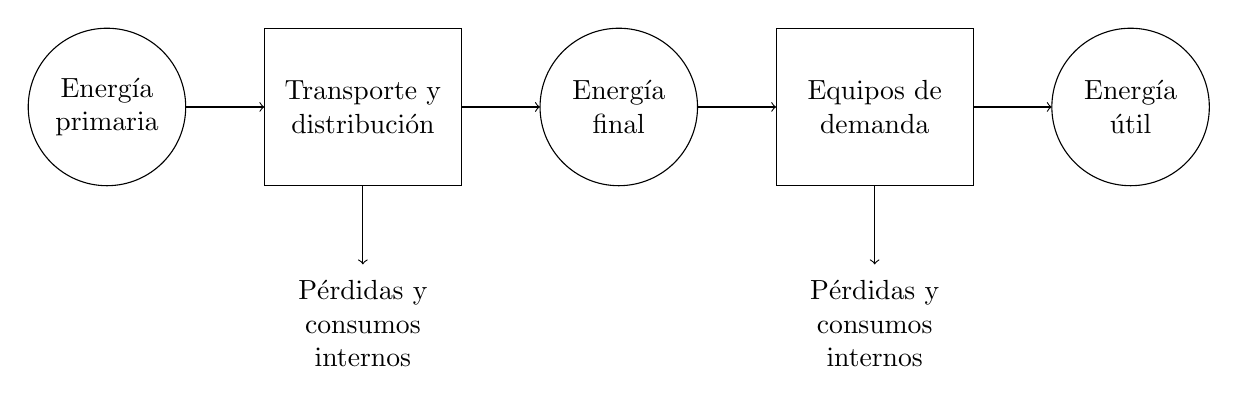
\begin{tikzpicture}
		\draw (0,0) circle (1cm);
		\node at (0,0) [align = center]{Energía\\primaria};
		\draw[->] (1,0) -- (2,0);
		
		\draw (2,-1) rectangle (4.5, 1);
		\node at (3.25,0) [align = center]{Transporte y\\distribución};
		\draw[->] (4.5,0) -- (5.5,0);
		
		\draw (6.5,0) circle (1cm);
		\node at (6.5,0) [align = center]{Energía\\final};
		\draw[->] (7.5,0) -- (8.5,0);
		
		\draw (8.5,-1) rectangle (11, 1);
		\node at (9.75,0) [align = center]{Equipos de\\demanda};
		\draw[->] (11,0) -- (12,0);
		
		\draw (13,0) circle (1cm);
		\node at (13,0) [align = center]{Energía\\útil};
		
		\draw[->] (3.25, -1) -- (3.25, -2);
		\node at (3.25, -2.75) [align = center]{Pérdidas y\\consumos\\internos};
		
		\draw[->] (9.75, -1) -- (9.75, -2);
		\node at (9.75, -2.75) [align = center]{Pérdidas y\\consumos\\internos};
	\end{tikzpicture}

\section{Formas prácticas de la energía.}
	Pueden ser el agua almacenada en un embalse, una barra de material fisionable o un combustible que al quemarse proporciona calor. No todos los combustibles proporcionan la misma cantidad de calor por unidad de masa (1 kg de gasolina $\neq$ 1 kg carbón).\\
	
	\indent Para poder relacionar y comparar unos con otros tendremos que referirnos a la cantidad específica de energía por unidad de masa (o de volumen), desprendida en un proceso de combustión, llamada \textbf{poder calorífico} o \textbf{densidad energética} o entalpía $\left(\dfrac{\textit{MJ}}{\textit{kg}}, \dfrac{\textit{MJ}}{\textit{l}}, \dfrac{\textit{MJ}}{\textit{Nm}^3}\right)$.
	
	\indent Los combustibles que dan agua como resultado de la combustión poseen dos poderes caloríficos, el inferior (\textbf{PCI}) y el superior (\textbf{PCS}). Las fuentes energéticas más buscadas son aquellas en las que la energía está 
	muy concentrada (mucha energía por unidad de masa).\\

	\begin{minipage}{\linewidth}
		\centering
		\begin{tblr}{
				cells = {c},
				cell{1}{1} = {r=2}{},
				cell{1}{2} = {c=2}{},
				hline{1,3,10} = {-}{},
				hline{2} = {2-3}{},
			}
			\textbf{Combustible} & \textbf{PCI}                                &                                     \\
			& $\dfrac{\textit{MJ}}{\textit{kg}}$ & $\dfrac{\textit{kWh}}{\textit{kg}}$ \\
			\textbf{Hidrógeno}   & 141.0                              & 39.2                                \\
			\textbf{Gas natural} & 46.4                               & 12.9                                \\
			\textbf{Gasolina}    & 43.3                               & 12.0                                \\
			\textbf{Gasóleo}     & 42.7                               & 11.9                                \\
			\textbf{Fuel-oil}    & 40.8                               & 11.3                                \\
			\textbf{Antracita}   & 35.1                               & 9.8                                 \\
			\textbf{Lignito}     & 25.6                               & 7.1                                 
		\end{tblr}
	\end{minipage}

\section{Concepto de eficiencia o rendimiento.}
	El rendimiento es un concepto termodinámico. En ingeniería suele utilizarse preferentemente la eficiencia, que establece la relación entre la energía útil y la primaria. A veces se llama COP (\textit{Coefficient of Performance})\\
	\indent Las distintas transformaciones energéticas implican una serie de pérdidas y consumos internos tanto en la generación como en el transporte.

	\begin{figure}[htbp]
		\begin{minipage}[t]{0.45\textwidth}
			\centering
			\begin{tblr}{
					cells = {c},
					cell{1}{1} = {c=2}{},
					hline{1,2,8} = {-}{},
				}
				{\textbf{Valores medios de eficiencias}\\\textbf{de diferentes tipos de centrales}} &      \\
				Hidroeléctrica                                                             & 85\% \\
				Térmica de Carbón                                                          & 40\% \\
				Nuclear                                                                    & 32\% \\
				Ciclo Combinado                                                            & 52\% \\
				Solar fotovoltaica                                                         & 18\% \\
				Cogeneración                                                               & 80\% 
			\end{tblr}
		\end{minipage}
		\hfill
		\begin{minipage}[t]{0.45\textwidth}
			\centering
			\begin{tblr}{
					cells = {c},
					cell{1}{1} = {c=2}{},
					hline{1,2,3,10} = {-}{},
				}
				{\textbf{Rendimiento de varios}\\\textbf{tipos de convertidores}} &               \\
				\textbf{Tipo de convertidor}                             & $\eta_{aprox}$ \\
				Motor de combustión                             & 30\%          \\
				Turbina de gas                                  & 29\%          \\
				Turbina Pelton                                  & 92\%          \\
				Célula de combustión                            & 80\%          \\
				Célula fotovoltaica                             & 12\%          \\
				Panel solar fototérmico                         & 70\%          \\
				Motor eléctrico                                 & 95\%          
			\end{tblr}
		\end{minipage}
	\end{figure}
	
	Aunque no es exactamente lo mismo, no se diferencia la energía mecánica de la energía eléctrica
	puesto que la conversión puede hacerse con factores cercanos a la unidad (el rendimiento de un
	generador síncrono puede llegar al 90\%)
	\[1\, \textit{kWh}_e \approx 1\, \textit{kWh}_m\]
	
	Sin embargo, no ocurre lo mismo con la energía eléctrica y la energía térmica. Pueden necesitarse
	hasta 3 o más $\textit{kWh}_t$ para obtener un $\textit{kWh}_e$.
	
\section{Unidades de energía.}
	La \textbf{Agencia Internacional de la Energía (AIE)} expresa sus balances de energía en una unidad
	común que es la \textbf{tonelada equivalente de petróleo (tep o toe)}:
	\begin{itemize}
		\item[-] Una tep se define como la energía liberada en la combustión de una tonelada de crudo de
		petróleo tipo de $10^4 \, \dfrac{\textit{kcal}}{\textit{kg}}$ de poder calorífico:
		
		\[1\,\textit{tep} = 10^7\,\textit{kcal}=41860\textit{MJ}\]
		\[0.086\,\textit{tep} = 1\, \textit{MWh}\]
		\[1\,\textit{tep} = 11.63\, \textit{MWh}\]
		
		\item[-] La conversión de unidades habituales a tep se hace en base a los poderes caloríficos inferiores
		de cada uno de los combustibles considerados.
	\end{itemize}
	
	La \textbf{tonelada equivalente de carbón (tec)} se define como la energía liberada en la combustión de
	una tonelada de hulla estándar de $7000 \, \dfrac{\textit{kcal}}{\textit{kg}}$ de poder calorífico. La equivalencia viene dada por: 
	\[1\,\textit{tec}=7\cdot10^6\,\textit{kcal} = 0.7\,\textit{tep}\]
	
	En las estadísticas de comercio internacional es frecuente hablar de \textbf{barriles de petróleo (bbl)}:
	\[1\,\textit{bbl} = 159\,\textit{l} = 0.146\,\textit{tep}\]
	
	La \textbf{U.S. Energy Information Administration (EIA)} utiliza el \textbf{BTU (British Thermal Unit)} como unidad de energía:
	\[1\,\textit{kWh} = 3412\,\textit{BTU}\]
	\[1\,\textit{therm} = 10^5\,\textit{BTU}\]
	
	\begin{minipage}{\linewidth}
		\centering
		\begin{tblr}{
				cell{1}{1} = {c=2}{},
				hline{1,2,9} = {-}{},
			}
			\textbf{Unidades de energía} &            \\
			1 \textit{tep}               & $10^7$ \textit{kcal} \\
			1 \textit{kcal}              & 4184 \textit{J}     \\
			1 \textit{MWh}               & 0.086 \textit{tep}  \\
			1 \textit{tec}               & 0.7 \textit{tep}    \\
			1 \textit{bbl}               & 0.146 \textit{tep}  \\
			1 \textit{kWh}               & 3412 \textit{BTU}   \\
			1 \textit{therm}             & $10^5$ \textit{BTU}   
		\end{tblr}
	\end{minipage}

\section{Unidades de energía en combustibles gaseosos.}
	Es frecuente referir el \textbf{PCI (poder calorífico inferior)} a la unidad de volumen ($\textit{m}^3$), pero si no están definidas las condiciones, carecería de significado.
	\begin{itemize}
		\item[-] \textit{Condiciones normales:} 
			corresponden a 0 \textdegree\textit{C} y 1 \textit{atm}. Se suele indicar con la letra \textit{N} al lado de la unidad de volumen, v.g. $3.4\,\textit{Nm}^3$.
			\[10^3\,{\textit{Nm}^3}_{Gas\ Natural} = 0.9\,\textit{tep}\]
			
		\item[-] \textit{Condiciones estándar:}
			corresponden a 15 \textdegree\textit{C} y 1 \textit{atm}. Se suele indicar con la letra \textit{S} al lado de la unidad de volumen, v.g. $3.4\,\textit{Sm}^3$.
			
		\item[-] \textit{Thermia (th):}
			unidad de energía, equivalente a 1 millón de calorías. Se usa en el suministro
			de gas natural para calcular las facturas. Como el gas suministrado tiene un poder calorífico algo
			variable, el cobro se hace en termias en vez de $\textit{m}^3$.\\
			Referido a un gas con PCS = $10^4\, \dfrac{\textit{kcal}}{\textit{Nm}^3} = 10\, \dfrac{\textit{th}}{\textit{Nm}^3}$
	\end{itemize}

\section{Consumo mundial de energía primaria.}
	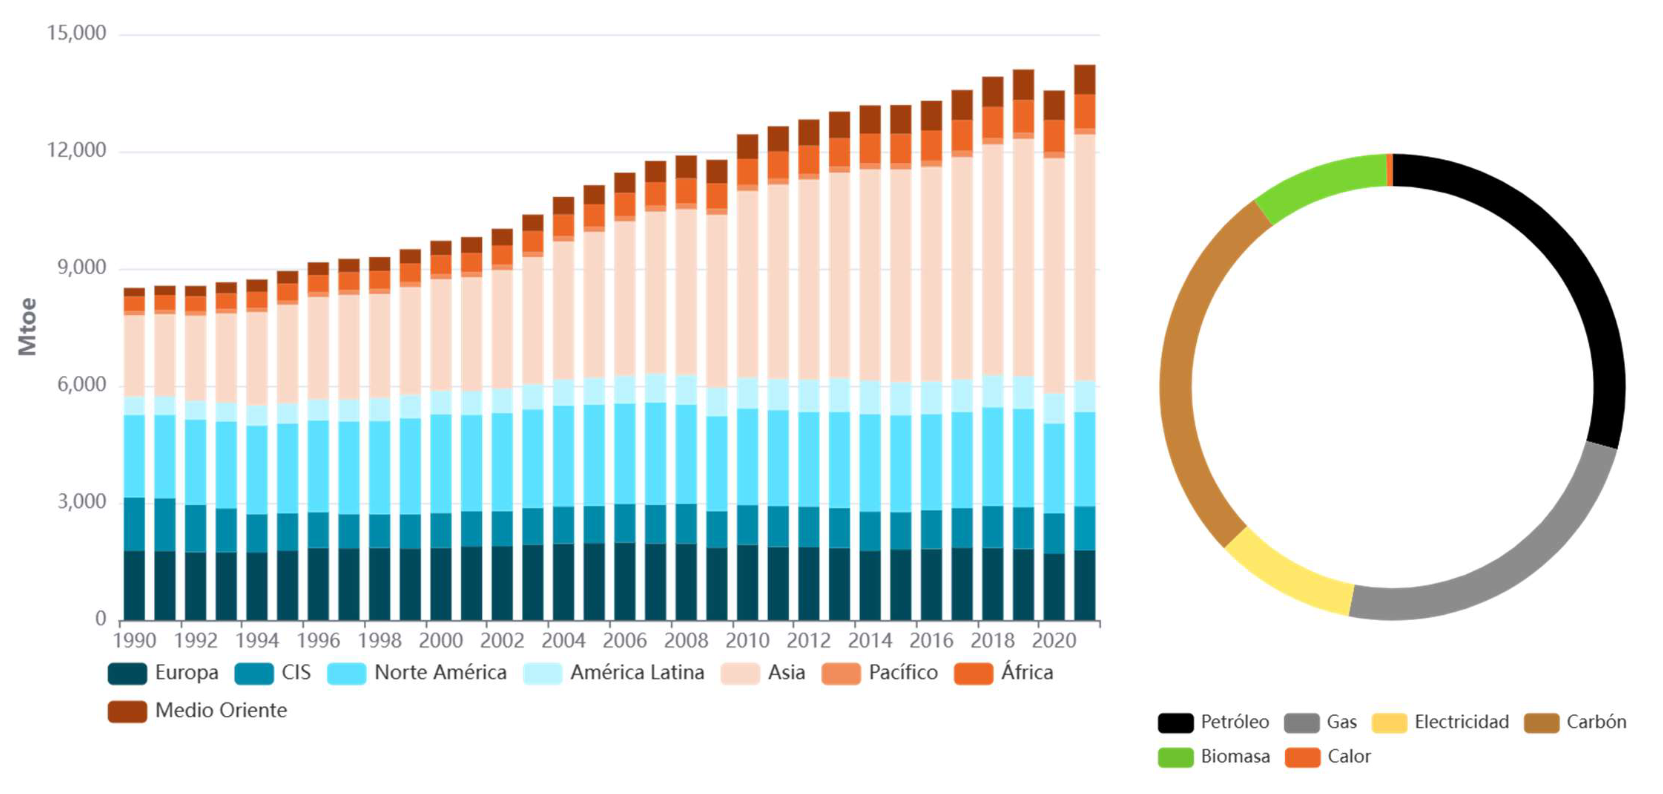
\includegraphics[width = 14cm, height = 6.68cm]{evolucionConsumo}
	
	El \textbf{WEC (World Energy Council}, fundado en 1923, considera tres
	escenarios hasta el 2020 en su estudio \textquotedblleft \textit{Energía para el mundo del mañana}\textquotedblright que publicó en 1993.
	En todos ellos se considera que para el año 2020 la población mundial será de 8100 millones
	(según Naciones Unidas). En el año 2022 hay 8.000 millones. Para el año 2030 se estima en 8.500
	millones.\\
	\indent Existen diversos escenarios atendiendo al balance entre crecimiento económico y orientación ecológica:
	\begin{itemize}
		\item[-] \textbf{Escenario de referencia}: 
			Crecimiento económico medio. La economía mundial crece
			moderadamente a una media del 3.3\% anual, resultando una demanda de energía primaria
			mundial en 2020 de 13.4 \textit{Gtep}, y una aportación de las renovables nuevas para ese año del 4.5\% (0.6 \textit{Gtep}).\\
			Considerando este estudio y con estos niveles de consumo de energía primaria y unos valores
			de reserva aproximados a los indicados anteriormente, se puede estimar el tiempo de duración de los
			distintos combustibles en años: 
			
			\begin{table}[H]
				\renewcommand{\arraystretch}{1.2}
				\centering
				\begin{tabular}{cc}
					\hline
					\textbf{Fuente de Energía} & \textbf{Duración (años)} \\
					\hline
					Petróleo & 42,2 \\
					Carbón & 224 \\
					Gas Natural & 62,2 \\
					Uranio & 100 \\
					\hline
				\end{tabular}
			\end{table}
			
			Las reservas totales de uranio se sitúan en unos 6,14 millones de toneladas. La demanda de las 442 unidades
			nucleares en funcionamiento (año 2011) fue de 68.875 toneladas de uranio.
			
		\item[-] \textbf{Escenario de alto crecimiento económico}: 
			el crecimiento económico es del 3,8\% y la demanda de energía primaria en el 2020 de unas 17 \textit{Gtep} y una aportación de las renovables nuevas del 4.5\% (0.8 \textit{Gtep}).
			
		\item[-] \textbf{Escenario ecológico:} 
			crecimiento económico medio con orientación ecológica. El crecimiento se supone del 3.3\%, pero la demanda de energía primaria crece sólo a 11.3 \textit{Gtep} en el 2020, y una aportación de las renovables del 11.5\% (1.3 \textit{Gtep}).
	\end{itemize}

	\indent Todos los estudios indican un \textbf{crecimiento potencial de las renovables}. Según estimaciones de Naciones Unidas, se calcula la aportación de las renovables en el 30\% de las necesidades mundiales
	en el 2025, y el 45\% en el 2050.

	Evolución del consumo energético en España:\\
	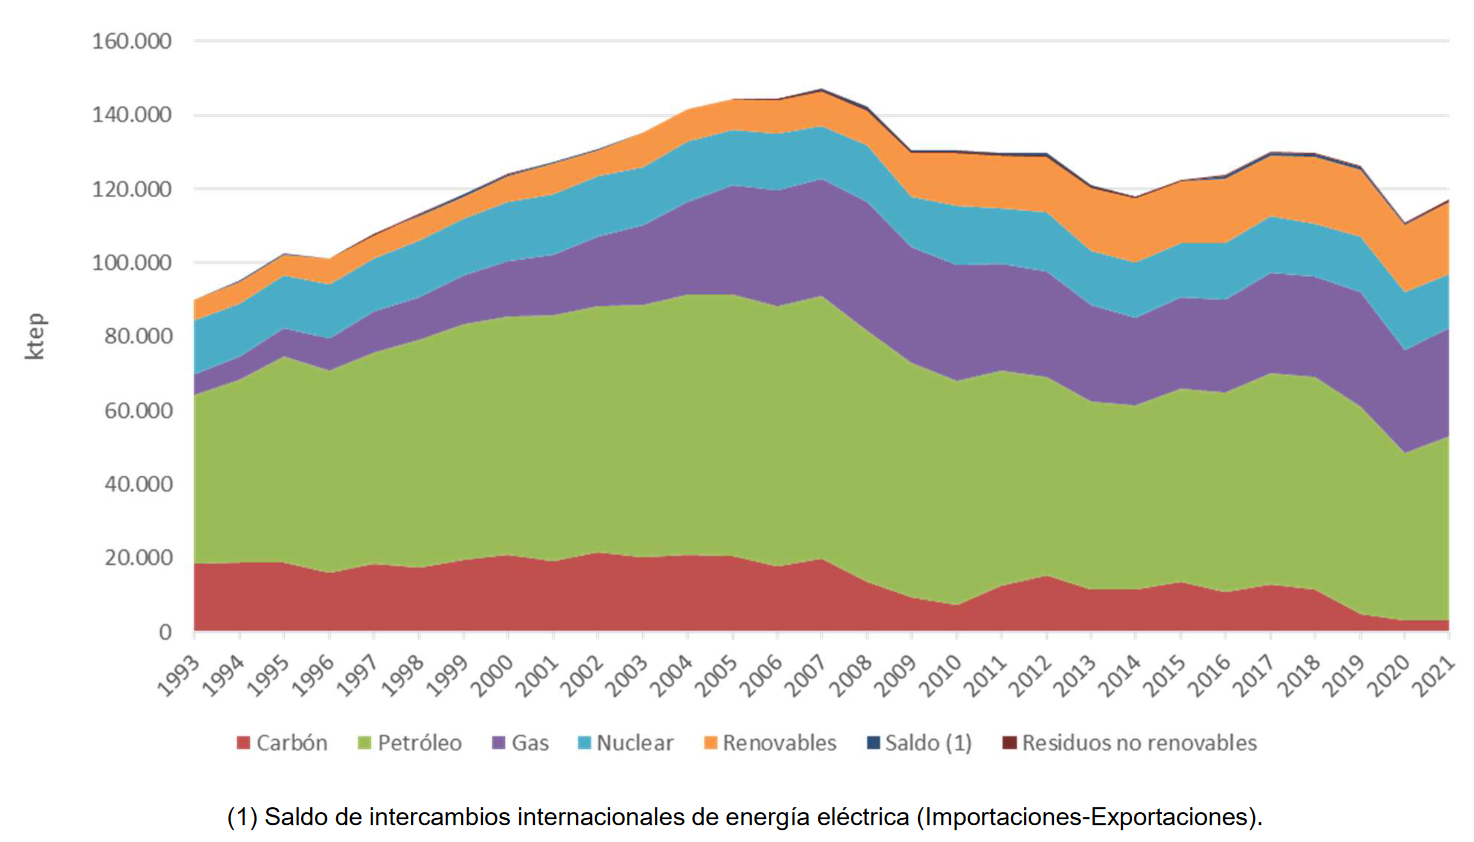
\includegraphics[width = 14cm, height = 7cm]{consumoEspaña}

\section{Intensidad energética primaria y de energía final.}
	\subsection{Intensidad energética primaria.}
		Se define como el cociente entre el consumo de energía primaria y el PIB en un año concreto. Tiene unidades de $\dfrac{\textit{ktep}}{\textit{M€}}$.\\
		\indent En España, a partir del 2005, se constató una mejora notable en la
		intensidad energética primaria, lo que significa que para producir una
		unidad de riqueza cada vez se necesita menor cantidad de energía (mayor
		eficiencia energética). Ha habido una ralentización del consumo energético y un
		crecimiento del PIB. España se encuentra en el puesto 34 de los 196 países.
		
	\subsection{Intensidad de energía final.}
		Se define como el cociente entre el consumo de energía final y el PIB.\\
		\indent La intensidad de energía final ha disminuido progresivamente. Esta mejora se debe sobre todo
		a las mejoras tecnológicas y de gestión, así como a la mejora de la estructura productiva y de la Ley de Energías Renovables y Eficiencia Energética.\\
		\indent En el año 2020 hubo una caída del PIB del 11\% junto con una bajada de consumo de energía primaria debido a la pandemia de COVID-19.
		
	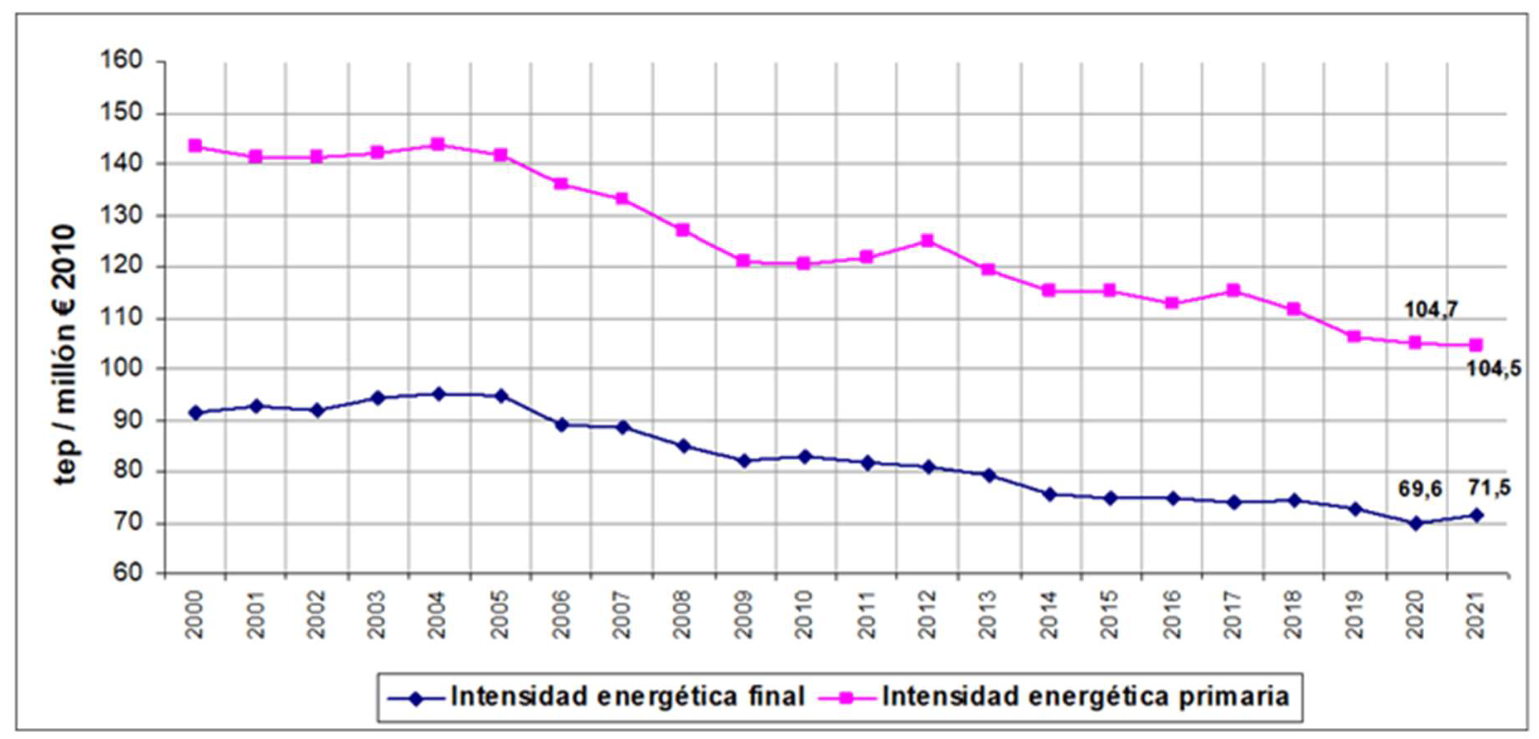
\includegraphics[width = 14cm, height = 7cm]{intensidadEnergiaEspaña}

\section{Contribución de las energías renovables a la reducción del consumo de energías primarias.}
	\subsection{Plan de fomento de las energías renovables (PFER, 2005-2010)}
		Objetivo para el 2010: Reducción del consumo de energía primaria un 12\%. A finales del 2010 el
		grado de cumplimiento fue del 11.3\%
	
	\subsection{Plan de fomento de las energías renovables (PANER, 2011-2020)}
		Objetivo para el 2020: Reducción del 20\% el consumo total de energía primaria (\textbf{cumplido}).

		\begin{table}[H]
			\centering
			\begin{tabular}{lccc}
				\hline
				\textbf{Fuente de Energía} & \textbf{Potencia Dic. 2019 (MW)} & \textbf{Potencia Dic. 2020 (MW)} & \textbf{$\Delta$19/20 (\%)} \\
				\hline
				$\uparrow$ Energías renovables & 58.269 & 62.517 & 7,3 \\
				\quad $\uparrow$ Eólica & 25.583 & 27.259 & 6,6 \\
				\quad $\uparrow$ Fotovoltaica & 8.973 & 11.547 & 28,7 \\
				\quad $=$ Otras renovables & 23.713 & 23.711 & -0,01 \\
				$\downarrow$ Carbón & 8.972 & 4.342 & -51,6 \\
				\hline
			\end{tabular}
		\end{table}
		
		\begin{table}[H]
			\centering
			\begin{tabular}{lccc}
				\toprule
				\textbf{Fuente de Energía} & \textbf{Gen. Bruta 2019 (GWh)} & \textbf{Gen. Bruta 2020 (GWh)} & \textbf{$\Delta$19/20 (\%)} \\
				\midrule
				Energías renovables & 100.988 & 113.008 & 11,9 \\
				\quad Eólica & 55.647 & 56.273 & 1,1 \\
				\quad Fotovoltaica & 9.420 & 15.552 & 65,1 \\
				\quad Otras renovables & 35.921 & 41.183 & 14,6 \\
				Carbón & 13.982 & 5.911 & -57,7 \\
				\bottomrule
			\end{tabular}
		\end{table}
		
	\subsection{Plan nacional integrado de energía y clima (PNIEC, 2011-2030)}
		Objetivos fijados para 2030:
		\begin{itemize}
			\item[-] 
				\textbf{Reducción de un 23\% de emisiones de gases de efecto invernadero} (GEI) respecto a 1990.
				\begin{itemize}
					\item 
						Emisiones totales brutas de GEI pasen de 319,3 $\textit{MtCO}_{2-eq}$ previstos para 2020 a 221,8 $\textit{MtCO}_{2-eq}$ en 2030. En lo que se refiere a generación eléctrica, reducción de 36 $\textit{MtCO}_{2-eq}$.
					\item 
						Las centrales de carbón cesan de aportar energía al sistema como tarde en 2030.
				\end{itemize}
				
			\item[-] 
				\textbf{Subir el uso de energías renovables a un 42\%} sobre el total de la generación mediante varias estrategias: bombas de calor, vehículo eléctrico, biocarburantes, sistemas de acumulación de energía eléctrica, etc.
				
			\item[-] 	
				\textbf{Mejora de la eficiencia energética en un 39.5\%} mediante:
				\begin{itemize}
					\item Renovación del parque edificatorio público.
					\item Auditorías energéticas.
				\end{itemize}
				
			\item[-] 
				\textbf{Aumentar el porcentaje de generación de energía eléctrica a un 74\%}. El Plan prevé para el año 2030 una potencia total instalada en el sector eléctrico según se muestra en la siguiente tabla.
				
				\begin{center}
					\begin{table}[H]
						\centering
						\begin{tabular}{lc}
							\textbf{Fuente de Energía} & \textbf{Capacidad (GW)} \\
							\hline
							Energía eólica & 50 \\
							Solar fotovoltaica & 39 \\
							Ciclos combinados de gas & 27 \\
							Hidráulica & 16 \\
							Bombeo & 9,5 \\
							Solar termoeléctrica & 7 \\
							Nuclear & 3
						\end{tabular}
					\end{table}
				\end{center}
				
				\quad La reducción del consumo de energía primaria propuesta en este PNIEC equivale a un 1,9\% anual desde 2017
				que, ligado a un incremento previsto del PIB en ese mismo periodo del orden del 1,7\%, tendrá como resultado
				una mejora de la intensidad energética primaria de la economía del 3,5\% anual hasta 2030.
				
			\item[-] 
				\textbf{Reducción de la dependencia energética:} la dependencia en energía primaria tiene importantes repercusiones económicas. Así, en el año 2017, el saldo del comercio exterior de energía fue desfavorable para nuestro país por valor de más de 20.000 \textit{M€}.\\
				Como resultado de las medidas contempladas en el PNIEC, 2021-2030, la ratio de dependencia energética de España disminuye 12 puntos porcentuales, pasando del 73\% en 2017 al 61\% en 2030.
				
				\begin{center}
					\begin{table}[H]
						\centering
						\begin{tabular}{lcccc}
							\toprule
							Año & 2015 & 2020* & 2025* & 2030* \\
							\midrule
							\textbf{Producción nacional} & 33,564 (27\%) & 37,499 (29\%) & 41,909 (35\%) & 40,646 (39\%) \\
							Carbón & 1,246 & 1,105 & 0 & 0 \\
							Productos petrolíferos & 236 & 146 & 147 & 148 \\
							Gas natural & 54 & 49 & 49 & 49 \\
							Nuclear & 14,903 & 15,118 & 15,118 & 6,500 \\
							Energías renovables & 16,873 & 20,611 & 26,150 & 33,501 \\
							Residuos no renovables & 252 & 470 & 445 & 448 \\
							\midrule
							\textbf{Neto importado/exportado} & 89,366 (73\%) & 91,008 (71\%) & 76,513 (65\%) & 63,453 (61\%) \\
							Carbón & 12,337 & 7,979 & 3,743 & 2,133 \\
							Productos petrolíferos & 52,809 & 55,473 & 49,155 & 40,498 \\
							Gas natural & 24,484 & 26,641 & 24,208 & 24,389 \\
							Electricidad & -11 & 762 & -1,202 & -3,448 \\
							Energías renovables & -253 & 153 & 610 & -119 \\
							\textbf{Total Energía Primaria} & 122,930 & 128,507 & 118,422 & 104,099 \\
							\bottomrule
						\end{tabular}
					\end{table}
				\end{center}
		\end{itemize}
		
\section{Evolución de la potencia renovable instalada en régimen regulado en España.}
	\begin{table}[H]
		\centering
		\begin{tabular}{cccccccc}
			\toprule
   Año & Solar FV & Solar Térmica & Eólica & Mini Hidráulica & Biomasa & Otras Renov. & Total \\
			\midrule
			1990 & & & 2 & 640 & & & 643 \\
			1995 & 1 & & 98 & 998 & 40 & & 1,137 \\
			2000 & 2 & & 2,296 & 1,466 & 148 & & 3,911 \\
			2005 & 47 & & 10,095 & 1,768 & 500 & & 12,410 \\
			2010 & 3,830 & 532 & 19,700 & 2,005 & 709 & & 26,776 \\
			2011 & 4,233 & 999 & 21,063 & 2,010 & 736 & 0 & 29,042 \\
			2012 & 4,524 & 1,950 & 22,630 & 2,012 & 810 & 0 & 31,927 \\
			2013 & 4,646 & 2,299 & 22,966 & 2,068 & 754 & 5 & 32,738 \\
			2014 & 4,655 & 2,299 & 22,984 & 2,092 & 793 & 5 & 32,828 \\
			2015 & 4,665 & 2,299 & 23,000 & 2,103 & 801 & 5 & 32,873 \\
			2016 & 4,672 & 2,299 & 23,063 & 2,105 & 805 & 5 & 32,949 \\
			2017 & 4,676 & 2,299 & 23,091 & 2,106 & 805 & 5 & 32,982 \\
			2018 & 4,699 & 2,299 & 23,191 & 2,098 & 821 & 5 & 33,113 \\
			2019 & 8,052 & 2,299 & 24,423 & 2,144 & 921 & 5 & 37,845 \\
			2020 & 10,748 & 2,299 & 26,845 & 2,145 & 1,023 & 5 & 43,064 \\
			2021 & 14,287 & 2,299 & 27,964 & 2,145 & 1,026 & 5 & 47,725 \\
			2022 & 19,785 & 2,304 & 29,994 & 2,145 & 1,024 & 5 & 70,452 \\
		\end{tabular}
	\end{table}

\section{Potencia instalada y evolución de la demanda en España.}
	\begin{table}[H]
		\renewcommand{\arraystretch}{1.2}
		\centering
		\begin{tabular}{lcc|cc|ccc}
			& \multicolumn{2}{c|}{Sistema peninsular} & \multicolumn{2}{c|}{Sistema no peninsular} & \multicolumn{3}{c}{Nacional} \\
			\cline{2-8}
			& MW & \%22/21 & MW & \%22/21 & MW & \%22/21 & 2024 (MW)\\
			\hline
			Hidráulica & 17,093 & 0.0 & 2 & 0.0 & 17,094 & 0.0 & 17,097 \\
			Hidroeólica & - & - & 11 & 0.0 & 11 & 0.0 & 11\\
			Eólica & 29,417 & 4.9 & 577 & 2.4 & 29,994 & 4.9 & 30,793 \\
			Solar fotovoltaica & 19,348 & 29.4 & 437 & 31.4 & 19,785 & 29.4 & 25,084\\
			Solar térmica & 2,304 & 0.0 & - & - & 2,304 & 0.0 & 2,304\\
			Otras renovables & 1,087 & 0.0 & 6 & 0.0 & 1,093 & 0.0 & 1,094\\
			Residuos renovables & 132 & 0.0 & 38 & 0.0 & 170 & 0.0 & 170\\
			\textbf{Renovables} & \textbf{69,381} & \textbf{9.1} & \textbf{1,071} & \textbf{12.4} & \textbf{70,452} & \textbf{9.1} & \\
			Turbinación bombeo & 3,331 & 0.0 & - & - & 3,331 & 0.0 & 3,331\\
			Nuclear & 7,117 & 0.0 & - & - & 7,117 & 0.0 & 7,117\\
			Carbon & 3,223 & -8.5 & 241 & - & 3,464 & -8.0 & 2,061\\
			Fuel + Gas & 8 & 0.0 & 2,400 & 0.0 & 2,408 & 0.0 & 8\\
			Ciclo combinado & 24,562 & 0.0 & 1,688 & - & 26,250 & 0.0 & 26,250\\
			Cogeneración & 5,593 & -0.3 & 50 & - & 5,643 & -0.3 & 5,631\\
			Residuos no renov. & 387 & -4.8 & 38 & 0.0 & 426 & -4.4 & 426\\
			\textbf{No Renovables} & \textbf{44,222} & \textbf{-0.8} & \textbf{4,418} & \textbf{0.0} & \textbf{48,639} & \textbf{-0.7} & \\
			\hline
			\textbf{Total} & \textbf{113,602} & \textbf{5.0} & \textbf{5,489} & \textbf{2.2} & \textbf{119,091} & \textbf{4.9} & \textbf{123,718}\\
		\end{tabular}
	\end{table}

\section{Balance de producción de energía eléctrica en España.}
	Datos en \textit{GWh}.
	\begin{table}[H]
		\renewcommand{\arraystretch}{1.2}
		\centering
		\begin{tabular}{l|cccccc}
			& 2018 & 2019 & 2020 & 2021 & 2022 & 2024\\
			\hline
			Hidráulica            & 34.117  & 24.719 & 30.632  & 29.626  &  17.863 & 146\\
			Eólica                & 49.581  & 54.245 & 54.906  & 60.526  &  61.176 & 134\\
			Solar fotovoltaica    &  7.766  &  9.252 & 15.302  & 20.981  &  27.864 & 171\\
			Solar térmica         &  4.424  &  5.166 &  4.538  &  4.706  &   4.123 & 6\\
			Hidroeólica           & 24      & 23     & 20      & 23      &  23     & 0\\
			Otras renovables      &  3.557  &  3.618 &  4.482  &  4.720  &   4.656 & 10\\
			Residuos renovables   &  874    &  890   &  726    &  878    &   878   & 2\\
			\textbf{Generación renovable}  & \textbf{100.344} & \textbf{97.913} & \textbf{110.605} & \textbf{121.459} & \textbf{116.583} & \\
			Turbinación bombeo    &   1.994 &  1.646 &   2.751 &   2.649 &   3.776 & 12\\
			Nuclear               &  53.198 & 55.824 &  55.758 &  54.041 &  55.984 & 169\\
			Ciclo combinado       &  30.044 & 55.242 &  44.023 &  44.500 &  68.138 & 70\\
			Carbón                &  37.277 & 12.671 &   5.021 &   4.983 &   7.765 & 7\\
			Motores diésel        &   3.178 &  2.836 &   2.399 &   2.517 &   2.548 & 6\\
			Turbina de gas        &   1.049 &  671   &   407   &   424   &   657   & 1\\
			Turbina de vapor      &   2.455 &  2.189 &   1.388 &   1.108 &   1.207 & 3\\
			Fuel + Gas            &  -0     & -0     &   0     &  -0     &   0     & \\
			Cogeneración          &  29.007 & 29.615 &  27.030 &  26.090 &  17.758 & 56\\
			Residuos no renovables &  2.435 &  2.222 &   2.016 &   2.239 &   1.900 & 4\\
			\textbf{Generación no renovable} & \textbf{160.637} & \textbf{162.915} & \textbf{140.794} & \textbf{138.552} & \textbf{159.732} & \\
			Consumos en bombeo    &  -3.198 & -3.027 &  -4.628 &  -4.318 &  -6.092 & \\
			Saldo I. internacionales & 11.102 &  6.862 &   3.280 &   852   & -19.802 & \\
			Generación total	  &&&&&&697\\
			\hline
			\textbf{Demanda en b.c.}       & \textbf{268.886} & \textbf{264.664} & \textbf{250.051} & \textbf{256.546} & \textbf{250.421} &\\
		\end{tabular}
	\end{table}

\section{Balance de intercambios internacionales.}
	Datos en \textit{GWh}.
	\begin{table}[H]
		\centering
		\begin{tabular}{lccc}
			\toprule
			\textbf{País} & \textbf{Importación (\%)} & \textbf{Exportación (\%)} & \textbf{Saldo} \\
			\midrule
			Francia & 54 & 46 & 145 \\
			Portugal & 23.7 & 76.3 & -775 \\
			Andorra & 0 & 100 & -35 \\
			Marruecos & 26.2 & 73.8 & -106 \\
			\bottomrule
		\end{tabular}
	\end{table}
	
\section{Evolución de las pérdidas de energía eléctrica en España}
	\begin{center}
		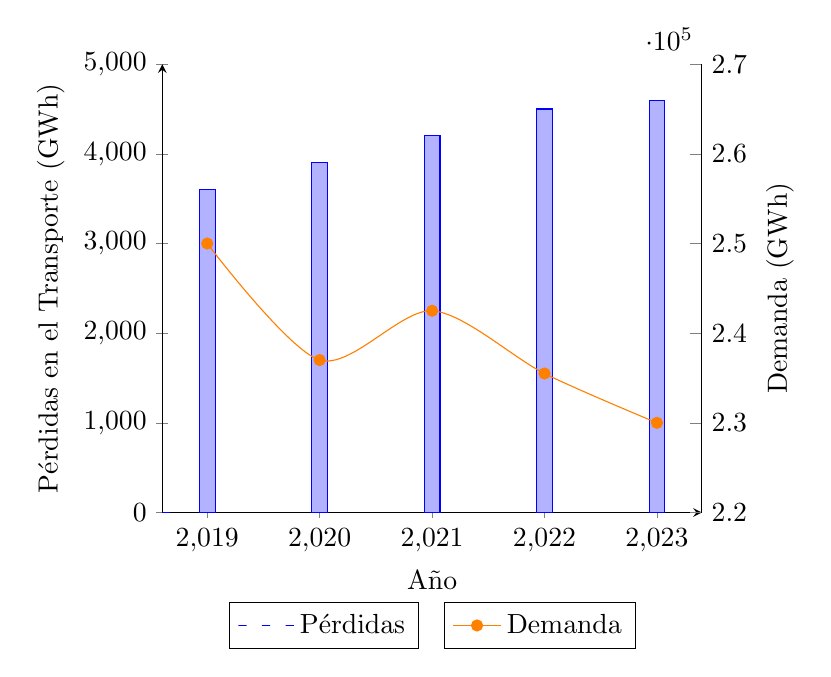
\begin{tikzpicture}
			\begin{axis}[
				xlabel={Año},
				ylabel={Pérdidas en el Transporte (GWh)},
				axis lines=left,
				ymin=0,
				ymax=5000,
				legend style={at={(0.3,-0.2)}, anchor=north},
				]
				
				% Datos en barras (azul)
				\addplot[blue, ybar, bar width=0.2cm, fill=blue!30] coordinates {
					(2018.6, 0)
					(2019, 3600)
					(2020, 3900)
					(2021, 4200)
					(2022, 4500)
					(2023, 4600)
					(2023.4, 0)
				};
				\addlegendentry{Pérdidas}
			\end{axis}
			
			\begin{axis}[
				axis y line*=right,
				ylabel={Demanda (GWh)},
				ymin=220000,
				ymax=270000,
				hide x axis,
				legend style={at={(0.7,-0.2)}, anchor=north},
				]
				
				% Datos en línea (naranja)
				\addplot[orange, smooth, mark=*] coordinates {
					(2019, 250000)
					(2020, 237000)
					(2021, 242500)
					(2022, 235500)
					(2023, 230000)
				};
				\addlegendentry{Demanda}
			\end{axis}
		\end{tikzpicture}	
	\end{center}

\section{Cobertura de la demanda de energía eléctrica en España.}
	Datos de Febrero de 2024, Red Eléctrica de España.
	\begin{figure}[H]
		\centering
		\begin{minipage}{.6\textwidth}
			\donutchart
			{
				15.16/cyan/Hidráulica,
				1.77/orange/Turbinación bombeo,
				21.65/yellow/Nuclear,
				0.95/red/Carbón,
				1.57/violet/Fuel + Gas,
				9.67/gray/Ciclo combinado,
				0.01/black/Hidroeólica,
				28.51/green5/Eólica,
				11.14/blue2/Solar fotovoltaica,
				0.77/red7/Solar térmica,
				1.26/violet3/Otras renovables,
				6.85/yellow7/Cogeneración,
				0.43/green/Residuos no renovables
			}
		\end{minipage}%
		\begin{minipage}{.4\textwidth}
			\begin{itemize}
				\item[\textcolor{cyan}    {\rule{1em}{1em}}] Hidráulica: 15.16\%
				\item[\textcolor{orange}  {\rule{1em}{1em}}] Turbinación bombeo: 1.77\%
				\item[\textcolor{yellow}  {\rule{1em}{1em}}] Nuclear: 21.65\%
				\item[\textcolor{red}     {\rule{1em}{1em}}] Carbón: 0.95\%
				\item[\textcolor{violet}  {\rule{1em}{1em}}] Fuel + Gas: 1.57\%
				\item[\textcolor{gray}    {\rule{1em}{1em}}] Ciclo combinado: 9.67\%
				\item[\textcolor{black}   {\rule{1em}{1em}}] Hidroeólica: 0.01\%
				\item[\textcolor{green5}  {\rule{1em}{1em}}] Eólica: 28.51\%
				\item[\textcolor{blue2}   {\rule{1em}{1em}}] Solar fotovoltaica: 11.14\%
				\item[\textcolor{red7}    {\rule{1em}{1em}}] Solar térmica: 0.77\%
				\item[\textcolor{violet3} {\rule{1em}{1em}}] Otras renovables: 1.26\%
				\item[\textcolor{yellow7} {\rule{1em}{1em}}] Cogeneración: 6.85\%
				\item[\textcolor{green}   {\rule{1em}{1em}}] Residuos no renovables: 0.43\%
			\end{itemize}
		\end{minipage}
	\end{figure}
	
\section{Emisiones y factor de emisión de $\mathbf{CO_2}$ equivalente asociado a la generación de energía eléctrica en España (2023).}
	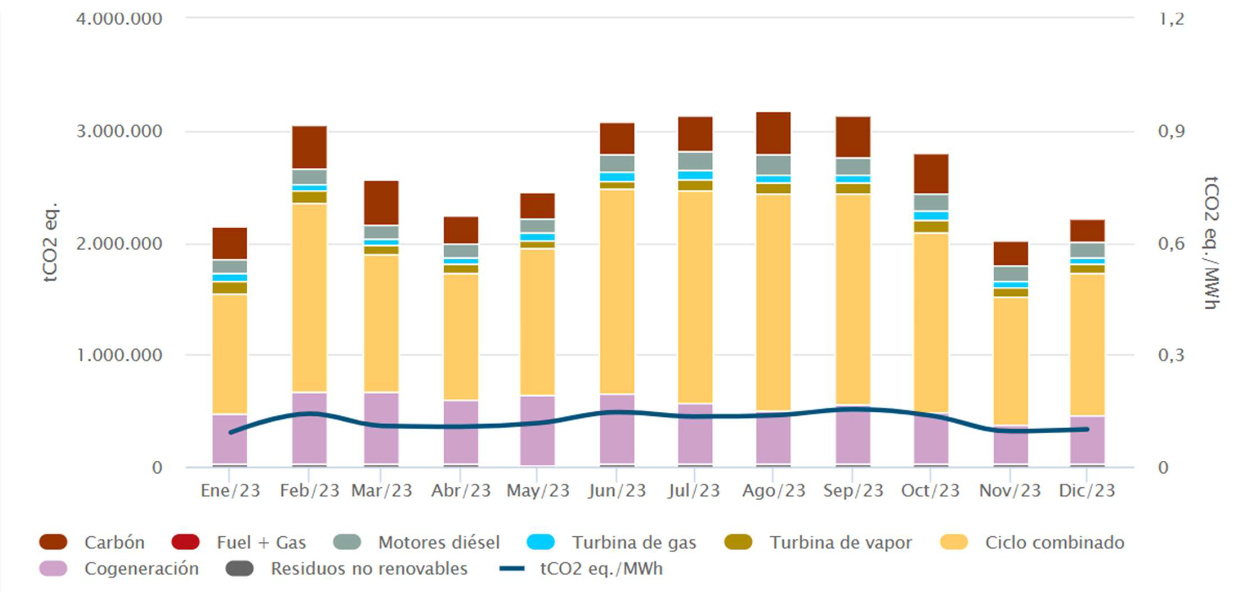
\includegraphics[width = 14cm, height = 7cm]{emisionesGeneracion}
	
\section{Clasificación de las centrales eléctricas según el tipo de energía primaria.}
	\begin{itemize}
		\item[-] \textit{Centrales hidroeléctricas:}
			\begin{itemize}
				\item Centrales hidráulicas convencionales.
				\item Centrales hidráulicas reversibles de bombeo.
			\end{itemize}
		\item[-] \textit{Centrales termoeléctricas:}
			\begin{itemize}
				\item Centrales de carbón
				\item Centrales de fuel-oil o gasoil.
				\item Centrales de ciclo combinado de gas natural.
				\item Centrales de cogeneración con gas natural.
			\end{itemize}
		\item[-] \textit{Centrales nucleares:}
			\begin{itemize}
				\item Centrales nucleares de agua a presión (PWR).
				\item Centrales nucleares de agua en ebullición (BWR).
			\end{itemize}
		\item[-] \textit{Centrales con energías renovables.}
			\begin{itemize}
				\item Centrales eólicas.
				\item Centrales termoeléctricas solares.
				\item Centrales fotovoltaicas.
				\item Centrales de biomasa (combustión y gasificación) y residuos sólidos urbanos (RSU).
				\item Centrales de energías marinas.
				\item Centrales geotérmicas.
				\item Centrales hidráulicas de tipo fluyente (desviaciones de ríos).
			\end{itemize}
	\end{itemize}
	
\section{Emplazamiento de las centrales eléctricas en España.}
	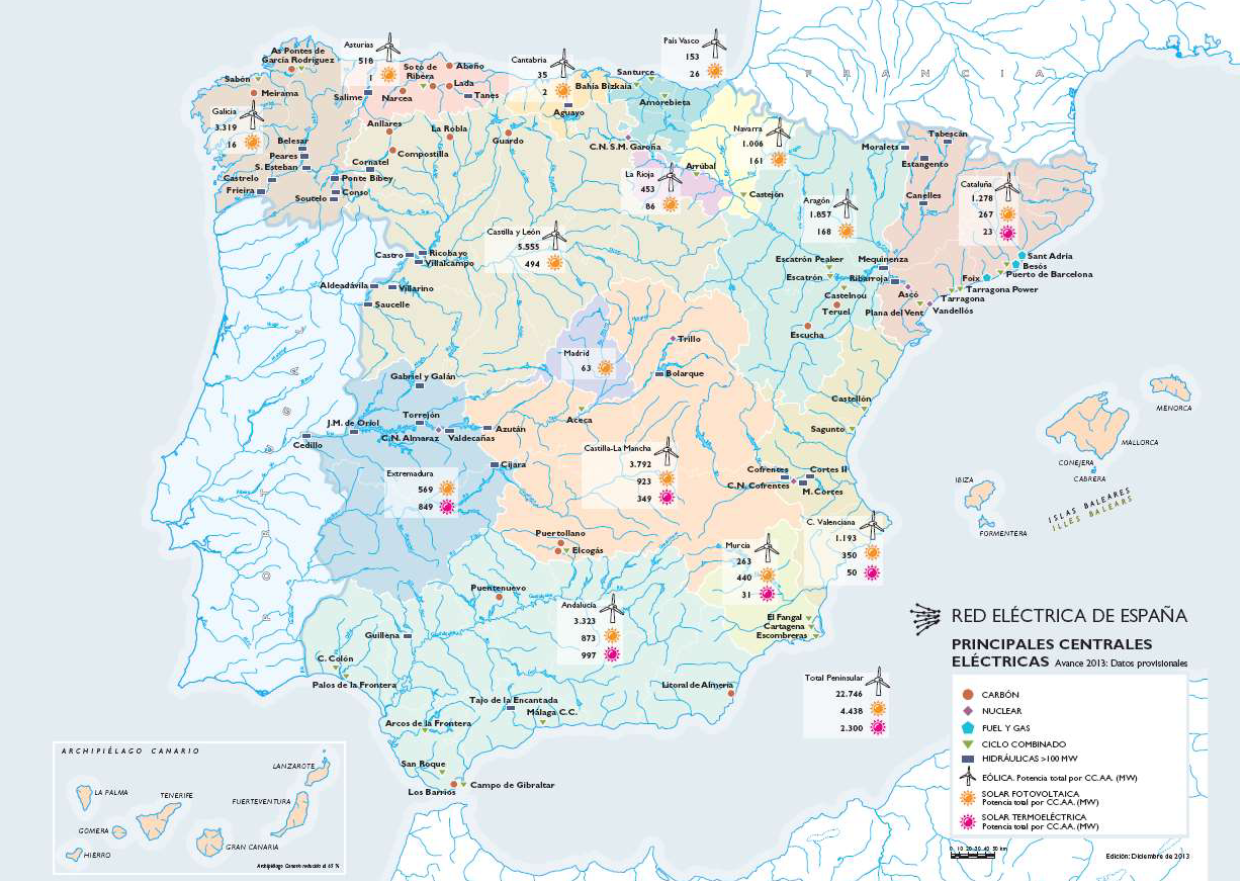
\includegraphics[width = 14cm, height = 9cm]{emplazamientoCentrales}
	
\section{Clasificación de las centrales termoeléctricas según el tipo de ciclo termodinámico.}
	\begin{itemize}
		\item[-] \textit{Ciclo de Rankine (Agua-Vapor):}
			para las centrales térmicas de carbón y nucleares de $>1000\,MW$ con \textbf{turbinas de vapor.}
		\item[-] \textit{Ciclo de Brayton-Erikson:}
			para centrales de gas natural con \textbf{turbinas de gas.}
		\item[-] \textit{Ciclo combinado Brayton-Rankine:} 
			centrales gas-aire y agua-vapor con \textbf{turbinas de gas natural y turbinas de vapor.}
		\item[-] \textit{Ciclos de Otto y Diesel:} 
			para cogeneración hasta $1\,MW$ con \textbf{motores de combustión interna.}
	\end{itemize}
	
\section{Clasificación de las centrales según la misión que realizan dentro del sistema eléctrico.}
	\begin{itemize}
		\item[-] \textit{Centrales de base:} 
			proporcionan la parte de energía que se consume de forma permanente en el sistema. \textbf{Centrales nucleares, térmicas, termosolares con acumulación, biomasa e hidráulicas de tipo fluyente.}
		\item[-] \textit{Centrales de puntas:}
			suministran la energía necesaria para atender las puntas de consumo. \textbf{Centrales hidroeléctricas, térmicas de gas natural y fuel-oil.}
		\item[-] \textit{Centrales intermedias:}
			suelen funcionar bajo programa (consigna de producción variable en función de la hora del día) de acuerdo con las previsiones de la demanda realizadas por las compañías. \textit{Centrales hidráulicas y térmicas de gas natural.}
		\item[-] \textit{Centrales de reserva:}
			entran en servicio en caso de avería o revisión de otras centrales.
		\item[-] \textit{Centrales de reserva rodante:}
			están en funcionamiento a baja carga. \textbf{Centrales de ciclo combinado e hidráulicas.}
		\item[-] \textit{Centrales de socorro:}
			pequeñas unidades transportables. \textbf{Grupos electrógenos de gasoil o fuel-oil.}
		\item[-] \textit{Centrales de acumulación:}
			consumen energía durante las horas de menor consumo. \textbf{Centrales hidráulicas de bombeo.}
	\end{itemize}
	
\section{Fuentes de energía primaria fósil.}
	\subsection{Petróleo (crudo de petróleo).}
		Es un aceite mineral de color oscuro o negro, menos denso que el agua y de un olor acre característico. Es una mezcla homogénea de compuestos orgánicos principalmente hidrocarburos insolubles en agua acompañados de azufre, oxígeno y nitrógeno en cantidades variables.
		
		\subsubsection{Formación del petróleo.}
			El petróleo en el subsuelo se encuentra atrapado en los pequeños espacios o poros de ciertas rocas
			sedimentarias, a la manera del agua en una esponja. Con el paso del tiempo, agua y petróleo van filtrándose a través de la roca madre, hasta encontrarse con una roca impermeable. La roca porosa está recubierta de una capa de roca impermeable. Si ésta tiene forma de bóveda, agua y petróleo se van acumulando gradualmente bajo ella.
			
			
			El crudo se separa del agua por
			diferencia de densidad y
			finalmente se sitúa en la parte
			superior de la roca porosa.
			A menudo se encuentra una capa
			de gas natural por encima de todo,
			coronando la bóveda.
			
			\begin{center}
				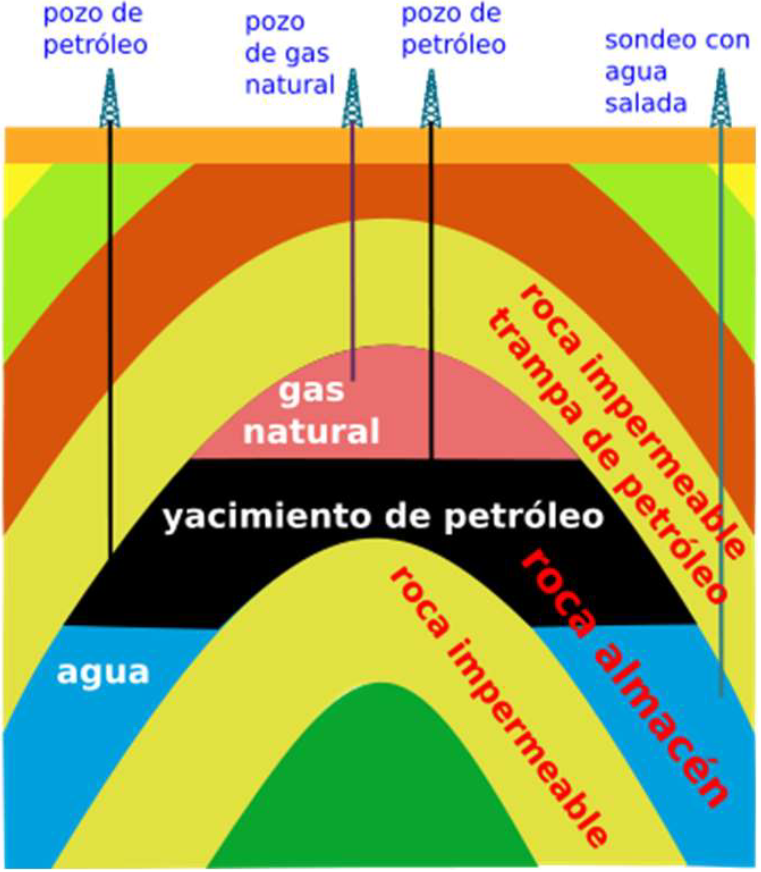
\includegraphics[width = 8cm, height = 10cm]{pozosPetroleo}
			\end{center}
			
		\subsubsection{Yacimientos de petróleo en el mundo.}
			\begin{center}
				\begin{tikzpicture}
					\def\printonlylargeenough#1#2{\unless\ifdim#2pt<#1pt\relax
						#2\printnumbertrue
						\else
						\printnumberfalse
						\fi}
					\newif\ifprintnumber
					\pie[rotate=90, text=legend, before number=\printonlylargeenough{6.86}, after number=\ifprintnumber\%\fi]{
						20.8/Venezuela,
						19.1/Resto del mundo,
						18.6/Arabia Saudí,
						9.63/Irán,
						8.08/Iraq,
						7.13/Kuwait,
						6.87/UAE,
						3.26/Libia: 3.26\%,
						2.61/Nigeria: 2.61\%, 
						1.78/Qatar: 1.78\%,
						0.85/Argelia: 0.85\%, 
						0.66/Angola: 0.66\%,
						0.45/Ecuador: 0.45\%
					}
				\end{tikzpicture}
			\end{center}
			
		\subsubsection{Extracción del petróleo.}
			\textbf{\textit{Extracción tradicional}}
				\begin{enumerate}
					\item 
						El crudo que brota espontáneamente por la presión interior del yacimiento recibe el nombre de \textbf{primario}.
					\item 
						Cuando la presión desciende se puede aumentar \textbf{inyectando agua, vapor de agua o gas en el interior}. Así se obtiene el \textbf{petróleo secundario}.
					
						La proporción entre el primario y el secundario depende de la porosidad de la roca y de la propia viscosidad del crudo. Suele ser un 25\% el primario.
					\item 
						Una vez explotado mediante este procedimiento se puede extraer más crudo reduciendo la viscosidad del petróleo \textbf{inyectando vapor de agua} para aumentar la temperatura, o por medio de \textbf{productos químicos} para diluirlo. Este es el \textbf{petróleo terciario.}
				\end{enumerate}
				
			\textbf{\textit{Fracking (fractura hidráulica).}}
			
			
				Es una técnica para posibilitar o aumentar la extracción de petróleo y gas del subsuelo. El proceso es el siguiente:
				\begin{enumerate}
					\item
						Se realiza la perforación vertical de un pozo, atravesando capas de roca y acuíferos, desde la plataforma en la superficie hacia donde se encuentra la capa de pizarra, que puede estar a varios kilómetros.
					\item 
						Antes de llegar a la capa de pizarra comienza la perforación horizontal o dirigida.
					\item 
						Dibujando una larga curva penetra finalmente en el estrato de pizarra, donde se extiende horizontalmente una media de 1-1.5 km. Como las distancias horizontales son muy largas, el proceso de fracking se lleva a cabo en varias etapas independientes.
					\item
						Una vez alcanzado el estrato deseado se utilizan explosivos para crear pequeñas grietas.
					\item 
						Se bombea un fluido, mezcla de agua y químicos, a elevada presión para abrir y extender las grietas.
					\item 	
						Al reducir la presión el fluido retorna a la superficie junto al gas y otras sustancias presentes en la roca, como metales pesados y partículas radiactivas.
					\item 
						La mezcla es procesada para separar todas las sustancias. Se estima que entre un 15 y un 80\% del fluido inyectado emerge de nuevo a la superficie, mientras el resto permanece bajo tierra.
				\end{enumerate}
				
				El proceso de fracking consume enormes cantidades de agua. Se ha calculado que se requieren entre 9000 y 29000 $m^3$ de agua para las operaciones de un solo pozo.
				
		\subsubsection{Alternativas a la producción de crudo de petróleo.}
			\begin{itemize}
				\item[-] \textit{Licuefacción del carbón.}
					También conocido como proceso de Pott-Broche. Es un proceso químico que converte el carbón directamente en una mezcla de hidrocarburos líquidos y luego se añade hidrógeno para realizar un hidrocraqueo en presencia de un catalizador. El producto obtenido es un crudo sintético que hay que refinar, consumiendo más hidrógeno. Las cantidades obtenidas aún son poco importantes.
				\item[-] \textit{Licuefacción indirecta.}
					Consiste en generar un gas de síntesis que luego es convertido en hidrocarburos líquidos mediante la reacción de Fischer-Tropsch.
				\item[-] \textit{Reservas de pizarras, arenas bituminosas o arenas de alquitrán.}
					Se separa el betún de la arena obteniendo un combustible fósil de baja graduación que require ser sometido a un proceso energético intensivo para convertirlo en crudo de petróleo sintético, parecido al crudo de petróleo convencional. Se hace añadiendo hidrógeno o quitando carbono. Muchas reservas pero poca producción.
			\end{itemize}
			
		\subsubsection{Grados API del petróleo.}
			El carácter más importante de los crudos es su densidad. Se puede dar en $g/cm^3$ o en grados API. Los grados API son una medida de cuánto pesa un producto de petróleo en relación al agua a temperaturas iguales. Si el producto del petróleo es más liviano que el algua y flota sobre ésta, su grado API es mayor que 10.
			
			
			\[1\,\dfrac{g}{cm^3} = 10^\circ API \text{ (crudos extra pesados (menor PCI))}\]
			
			\[0.77\,\dfrac{g}{cm^3} = 50^\circ API \text{ (crudos ligeros (mayor PCI))}\]
			
			
			Los grados API se utilizan para determinar el precio de un crudo determinado, ya que cuanto mayor es el valor en grados API mayor es la proporción de crudo utilizable. El 60\% de las reservas mundiales de petróleo tiene densidades inferiores a 33\textdegree API y contenidos de S superiores al 1.5\%. Por tanto, existe una oferta creciente de crudos pesados y ácidos.
			
		\subsubsection{Densidad relativa y gravedad específica.}
			\[\rho_r=\dfrac{\rho_{petroleo}[kg/m^3]}{\rho_{agua}[kg/m^3]} = GE\text{ (Gravedad específica)} = \rho\cdot g = \dfrac{m}{V}\cdot g\]
			
			\[GE = \dfrac{141.5}{API+131.5} \Rightarrow API=\dfrac{141.5}{GE}-131.5\]
			
		\subsubsection{Infraestructura de la red de transporte y distribución de productos petrolíferos.}
			Las empresas que cuentan con plantas de refino en españa son REPSOL, CAMPSA y Petronor, que forman las tres el grupo REPSOL-YPF (Yacimientos Petrolíferos Fiscales), CEPSA/Elf y BP.
			
			
			La distribuciuón y comercialización queda a cargo de CLH (Compañía Logística de Hidrocarburos), integrada en el grupo REPSOL. Se transporta en grandes buques petroleros, que pueden transportar hasta 300.000 toneladas.
			
		\subsubsection{Procedencia del crudo de petróleo en España.}
			\begin{table}[H]
				\begin{tabular}{llllll}
					\textbf{x1000 t}	&	\textbf{2000}	&	\textbf{2010}	&	\textbf{2020}	&	\textbf{2021}	&	\textbf{2022}	\\
					\hline
					Angola	&	664	&	1112	&	1696	&	679	&	2316	\\
					Argelia	&	1476	&	1010	&	827	&	1660	&	3172	\\
					Guinea Ecuatorial	&	0	&	0	&	735	&	1065	&	1238	\\
					Libia	&	6901	&	6826	&	1966	&	6270	&	4997	\\
					Nigeria	&	9165	&	5579	&	10840	&	10275	&	8123	\\
					\textbf{Total África}	&	\textbf{22804}	&	\textbf{18872}	&	\textbf{17888}	&	\textbf{21251}	&	\textbf{20608}	\\
					\hline
					Brasil	&	30	&	667	&	3070	&	2063	&	5401	\\
					Canadá	&	0	&	169	&	523	&	1435	&	2670	\\
					Colombia	&	0	&	74	&	456	&	145	&	974	\\
					Estados Unidos	&	0	&	0	&	3095	&	4096	&	6639	\\
					México	&	7622	&	5928	&	8443	&	7648	&	6125	\\
					Venezuela	&	1562	&	789	&	1403	&	0	&	727	\\
					\textbf{Total América}	&	\textbf{9214}	&	\textbf{7699}	&	\textbf{17397}	&	\textbf{15688}	&	\textbf{23459}	\\
					\hline
					Azerbaiyán	&	138	&	750	&	1769	&	1342	&	1942	\\
					Kazajistán	&	0	&	557	&	4519	&	4201	&	3298	\\
					Noruega	&	249	&	691	&	996	&	1600	&	1031	\\
					Reino Unido	&	2039	&	405	&	1017	&	502	&	1104	\\
					Rusia	&	5141	&	6665	&	979	&	2569	&	698	\\
					\textbf{Total Europa y Eurasia}	&	\textbf{8282}	&	\textbf{9331}	&	\textbf{10518}	&	\textbf{11540}	&	\textbf{9230}	\\
					\hline
					Arabia Saudí	&	6628	&	6571	&	5542	&	3942	&	4773	\\
					Iraq	&	5995	&	1905	&	3507	&	3751	&	5212	\\
					Irán	&	3880	&	7671	&	0	&	0	&	0	\\
					\textbf{Total Oriente Medio}	&	\textbf{17157}	&	\textbf{16559}	&	\textbf{9049}	&	\textbf{7693}	&	\textbf{10298}	\\
					\hline
					\textbf{Total Mundo}	&	\textbf{57457}	&	\textbf{52461}	&	\textbf{54852}	&	\textbf{56172}	&	\textbf{63596}	\\
					\hline
					Saldo Producción	&	12580	&	12758	&	-5407	&	-4919	&	-2437	\\
					\textbf{Total Saldo importador}	&	\textbf{70037}	&	\textbf{65219}	&	\textbf{49445}	&	\textbf{51253}	&	\textbf{61158} \\
					\hline
					
				\end{tabular}
			\end{table}
			
		\subsubsection{Refino y obtención de productos derivados del crudo de petróleo.}
			El petróleo, tal como se extrae del \textbf{yacimiento}, no tiene aplicación práctica alguna. Por ello se separa en diferentes \textbf{fracciones} que sí son de utilidad. Este proceso se realiza en \textbf{refinerías}.
			
			
			Una \textbf{refinería} es una instalación industrial en la que se transforma el petróleo crudo en productos útiles para las personas. El conjunto de operaciones que se realizan en las refinerías para conseguir estos productos son denominados \textbf{procesos de refino}.
			
			
			La industria del \textbf{refino} tiene como finalidad obtener del petróleo la mayor cantidad posible de productos de calidad bien determinada, que van desde gases ligres, como el \textbf{propano} y el \textbf{butano}, hasta las fracciones más pesadas, \textbf{fuel-oil} y \textbf{asfaltos}, pasando por otros productos intermedios como las \textbf{gasolinas}, el \textbf{gasoil} y los \textbf{aceites lubricantes}.
			
			
			\textit{Refinería de REPSOL en Puertollano, Ciudad Real:} es la mayor refinería de España, con una capacidad de destilación de crudo de \textbf{7.5 millones} de toneladas al año.
			
			
			\textit{Proceso de refino:}
			\begin{enumerate}
				\item Análisis del petróleo, ya que no todos los petróleos son iguales ni de todos se pueden extraer las mismas sustancias.
				\item Refinados piloto para experimentar a pequeña escala todas las operaciones de refino.
				\item Destilación fraccional: mediante calor se separan los diversos componentes del crudo en una columna:
				\begin{enumerate}
					\item Se sube la temperatura a $370^\circ C$.
					\item Las fracciones más pesadas se quedan en el fondo:
					\begin{itemize}
						\item Fuel-oil.
						\item Aceites lubricantes.
						\item Ceras y parafinas.
						\item Betunes y asfaltos.
						\item Coque de petróleo.
					\end{itemize}
					\item Añadiendo crudo recalentado y aplicando tratamientos se obtienen los gasóleos de motor y calefacción
					\item En el siguiente nivel se obtienen los querosenos: carburantes de aviación y aceites combustibles.
					\item En el nivel siguiente se obtienen las naftas: materia prima petroquímica.
					\item En el último nivel se obtienen las gasolinas.
					\item Los vapores que suben son los gases licuados del petróleo (GLPs): propano y butano.
				\end{enumerate}
				\begin{figure}
					\centering
					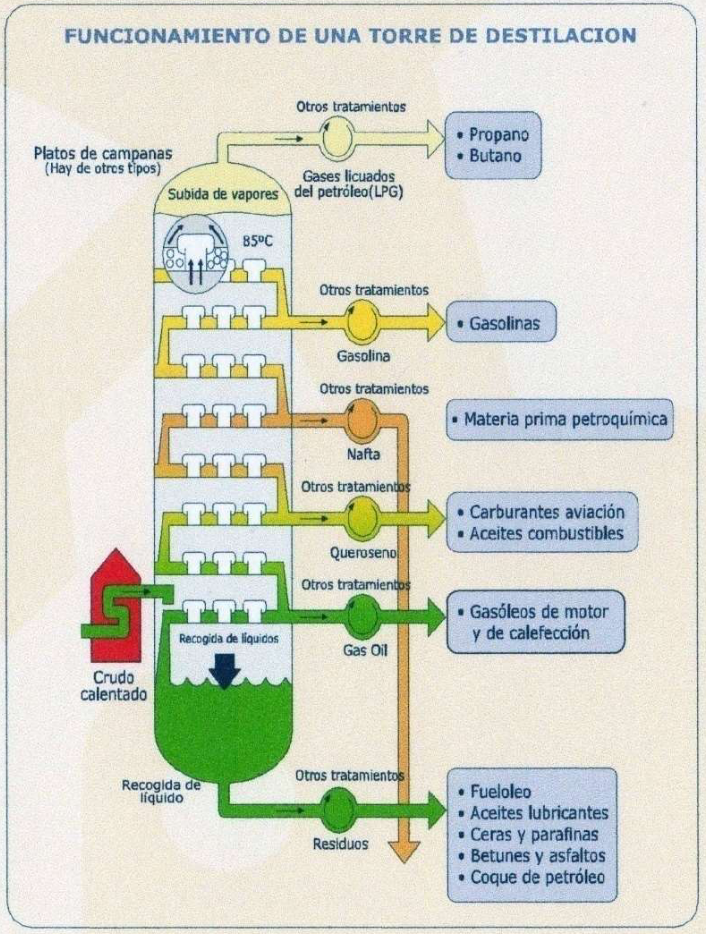
\includegraphics[width=0.6\linewidth]{res/tema1/destilacionPetroleo}
					\caption{Destilación del petróleo.}
					\label{fig:destilacionpetroleo}
				\end{figure}
				 
			\end{enumerate} 
		
		\subsubsection{Conversión de fuelóleos y residuos pesados.}
			Para la conversión del fuelóleo en destilados (gasóleos con bajo contenido en azufre), se han
			desarrollado técnicas como las siguientes:
			\begin{itemize}
				\item \textbf{Cracking catalítico en lecho fluido (FCC):} se utiliza ampliamente para convertir hidroccarburos de cadena larga en gasolina, sin adición de hidrógeno.
				\item \textbf{Hidrocraqueo:} es un proceso en dos fases que combina el craqueo catalítico y la
				hidrogenación, y por medio del cual las fracciones de destilado se descomponen en presencia de
				hidrógeno y catalizadores especiales dando lugar a productos de más valor.
			\end{itemize}
			
			
			En España hay 6 unidades de FCC y 1 de hidrocraqueo. El residuo pesado de una refinería disminuye en un 50\% con estas instalaciones.
			
			
			Técnicamente, la solución más correcta es la gasificación de los residuos sólidos y líquidos a través de la cual se produce \textbf{gas de síntesis}: $CO$ + $H_2$. Parte del hidrógeno se separa para ser utilizado en procesos de desulfuración o en plantas químicas, y el resto alimenta una central IGCC (gasificación + ciclo combinado).
			
		\subsubsection{Centrales termoeléctricas de fuel-oil y gasoil.}
			El combustible líquido se almacena en grandes tanques
			cilíndricos de superficie, construidos de chapa de acero
			al carbono soldada.
			
			
			Son muy viscosos a la temperatura ambiente y deben
			ser precalentados para que fluidifique y poder
			bombearlos desde los tanques hasta la central, siendo
			inyectado posteriormente en quemadores adecuados en
			una caldera o motor de combustión interna.
			
			
			Tan sólo un 5\% de la electricidad que se consume en
			España procede de centrales alimentadas con
			combustible líquido. Esta electricidad se emplea para cubrir las puntas de
			demanda. También se usan en sistemas no peninsulares (Islas Baleares y Canarias).
			
			
			Las centrales térmicas de carbón consumen fuel-oil o
			gasoil para precalentar el hogar en un arranque frío.
			
	\subsection{Gas natural.}
		Se encuentra en 2 tipos de yacimientos:
		\begin{itemize}
			\item Yacimientos de gas individualizado.
			\item Yacimientos asociados a los del petróleo.
		\end{itemize}
		
		
		Está principalmente compuesto por metano y etano.
		
		
		La densidad relativa del gas natural, tomando el aire
		como referencia, es de 0.6 a 0.66, es decir, es menos
		denso o pesado que el aire.
		
		
		Su poder calorífico, o cantidad de calor desprendida en
		la combustión completa por unidad de volumen, es de
		6.6 a $12\,\dfrac{te}{m^3}$ ($9.000 \dfrac{kcal}{Nm^3} = 37,6 \dfrac{MJ}{Nm^3}$).
		
		\subsubsection{Índice de Wobbe.}
			\[IW_{superior} = \dfrac{PCS}{\sqrt{GE}} = \dfrac{\text{Poder calorífico superior} \left(\dfrac{kcal}{Nm^3}\right)}{\sqrt{\text{Gravedad específica del gas}}}\]
			\[IW_{inferior} = \dfrac{PCS}{\sqrt{GE}} = \dfrac{\text{Poder calorífico inferior} \left(\dfrac{kcal}{Nm^3}\right)}{\sqrt{\text{Gravedad específica del gas}}}\]
			\[GE = \dfrac{\text{Densidad absoluta del gas natural} = 0.743 \dfrac{kg}{Nm^3}}{\text{Densidad absoluta del aire} = 1.2928 \dfrac{kg}{Nm^3}} = 0.5747\]
			\[PCS_{GN} = 10000 \dfrac{kcal}{Nm^3}\]
			\[PCI_{GN} = 9000 \dfrac{kcal}{Nm^3}\]
			\[IW_{superior} = \dfrac{10000}{\sqrt{0.5747}} = 13190.8 \dfrac{kcal}{Nm^3}\]

		\subsubsection{Reservas y producción.}
			\begin{center}
				\begin{tikzpicture}
					\def\printonlylargeenough#1#2{\unless\ifdim#2pt<#1pt\relax
						#2\printnumbertrue
						\else
						\printnumberfalse
						\fi}
					\newif\ifprintnumber
					\pie[rotate=90, text=legend, before number=\printonlylargeenough{6.77}, after number=\ifprintnumber\%\fi]{
						41.5/Oriente medio,
						32.61/Eurasia,
						7.83/África,
						6.78/Asia,
						4.48/Norteamérica: 4.48\%,
						3.90/América del sur: 3.90\%,
						2.90/Europa: 2.90\%
					}
				\end{tikzpicture}
			\end{center}
			
		\subsubsection{Tipos de extracción de gas no convencionales.}
			\begin{itemize}
				\item \textbf{Shale gas: procedente de pizarras y esquistos.}
					Son formaciones minerales procedentes de sedimentos ricos en arcillas , de grano fino pero bastante impermeables que se almacenan en capas paralelas que suelen contener gas natural. Las propiedades de estas rocas hacen que sea difícil extraer el gas natural, ya que para liberarlo es necesario fracturar la roca mediante Fracking.
				\item \textbf{Tight sand gas accumulations: gas en arenas de baja permeabilidad.}
					Como consecuencia de la baja permeabilidad de estas acumulaciones de arena, el gas natural queda atrapado en ellas sin poder ascender a capas más superficiales. Al igual que ocurre con el “shale gas” es necesario fracturar esta estructura para extraer el gas.
				\item \textbf{Coalbed methane (CBM): metano en capas de carbón.}
					De la misma manera que podemos encontrar el gas natural asociado al petróleo, también podemos encontrarlo asociado al carbón. Antiguamente esto suponía un problema a la hora de extraer el carbón en las minas, por su peligrosidad. Actualmente se recupera este gas liberado en la extracción de carbón y se conduce a los gasoductos.
			\end{itemize}
			
		\subsubsection{Consumo de gas natural en España.}
			\begin{table}[H]
				\renewcommand{\arraystretch}{1.2}
				\begin{tabular}{lrrrrrrr}
					\hline
					\textbf{Mercados} & \textbf{1990} & \textbf{2000} & \textbf{2010} & \textbf{2020} & \textbf{2021} & \textbf{2022} & $\mathbf{\Delta \%}$ \\
					\hline
					1. Doméstico comercial						& 10771 & 34755 & 64328 & 58819 & 63330 & 54810 & -13.5\\
					$\,\,\,\,\,\,$ Gas Natural						& 7578  & 34221 & 64279 & 58819 & 63330 & 54810 & -13.5\\
					$\,\,\,\,\,\,$ Gas manufacturado de gas natural	& 2604  & 31    & 0     & 0     & 0     & 0     & 0    \\
					$\,\,$ 1.1. Subtotal gas natural			& 10182 & 34253 & 64279 & 58819 & 63330 & 54810 & -13.5\\
					$\,\,\,\,\,\,$ Aire propanado					& 66    & 502   & 49    & s.d.  & s.d.  & s.d.  & s.d. \\
					$\,\,$ 1.2. Subtotal otros gases			& 589   & 502   & 49    & s.d.  & s.d.  & s.d.  & s.d. \\
					2. Industrial								& 44166 & 144994& 194089& 212316& 224700& 171550& -23.7\\
					3. Centrales eléctricas						& 2254  & 10379 & 135625& 88900 & 90400 & 138006& 52.7 \\
					4. Usos no energéticos						& 4835  & 6131  & 6131  & s.d.  & s.d.  & s.d.  & s.d. \\
					5. Gas natural vehicular					& s.d.  & s.d.  & s.d.  & s.d.  & s.d.  & s.d.  & s.d. \\
					\hline
					Total										& 62026 & 196258& 400174& 360035& 378430& 364366& -3.7\\
					Total (bcm)									& 5.3   & 16.8  & 34.4  & 30.9  & 32.5  & 31.3  & -   \\
					\hline
				\end{tabular}
			\end{table}
			
		\subsubsection{Procedencia del gas natural en España.}
			\begin{table}[H]
				\renewcommand{\arraystretch}{1.2}
				\begin{tabular}{lrrrr}
					\hline
					\textbf{GWh}  & \textbf{2010} & \textbf{2020} & \textbf{2021} & \textbf{2022}\\
					\hline
					Angola				&        & 4056   & 4128   & 3103\\
					Argelia				& 134159 & 106205 & 177990 & 106499\\
					Camerún				&        & 956    & 0      & 3179\\
					Egipto				& 32728  & 968    & 3906   & 15053\\
					EE.UU.				&        & 57117  & 60646  & 128917\\
					Francia				& 1851   & 22227  & 20224  & 19062\\
					Guinea Ecuatorial	& 0      & 10569  & 8890   & 5943\\
					Nigeria				& 86993  & 44195  & 47690  & 61726\\
					Noruega				& 37626  & 18310  & 11762  & 4022\\
					Omán				& 1931   & 0      & 0      & 5896\\
					Perú				& 7164   & 1875   & 865    & 1920\\
					Portugal			& 0      & 1857   & 3561   & 4685\\
					Qatar				& 65533  & 32248  & 26169  & 15429\\
					Rusia				&        & 38081  & 36197  & 56021\\
					Trinidad y Tobago	& 36972  & 24081  & 12270  & 13569\\
					\hline
					Total importaciones	& 412928 & 365226 & 415625 & 446208\\
					Total GNL			& 312905 & 226959 & 226571 & 319030\\
					Total GN			& 100023 & 136267 & 189054 & 127178\\
					Total exportaciones & 12914  & 13663  & 35756  & 68214\\
					\hline
				\end{tabular}
			\end{table}
			
			El fracking en España podría ser una realidad: habría gas para 70 años de consumo.
			Hasta ahora, en España solo hay permisos de investigación y no existe ninguna concesión, ya
			que los proyectos están sometidos a evaluaciones de impacto medioambiental.